To formalize the concepts of multi agent systems different types of logics are used, such as propositional, modal, temporal and dynamic logics. I this section these logics, their properties and introduced operators will be briefly discussed. Describing the details about interpretations and models of each individual logic is not the purpose of this section and is left out for further reading.

Propositional logic is the simplest one and serves as a fundament for logics discussed further in this section. It is used for representing factual information and in our case is most suitable to model the agent's environment. Formulas in this logic language consist of atomic propositions (known facts about the world) and truth-functional connectives: $\land,\lor,\neg,\rightarrow$ which denote "and" "or" "not" and "implies" respectively. \cite{Enderton_72} 

Modal logic extends propositional logic by introducing two different modes of truth: possibility and necessity. In the study of agents, it is used to give
meaning to concepts such as belief and knowledge. Syntactically modal operators in modal logic languages are defined as $\Diamond$  for possibility and 
$\Box$ for necessity. The semantics of modal logics is traditionally given in terms of sets of the so-called possible worlds. A world here can be interpreted as a possible state of affairs or sequence of states of affairs (history). Different worlds can be related via a binary accessibility relation, which tells us which worlds are are within the realm of possibility from the standpoint of a given world. In the sense of the accessibility relation a condition is assumed possible if it is true somewhere in the realm of possibility and it is assumed necessary if it is true everywhere in the realm of possibility. \cite{Saul_63}

Dynamic logic is also can be referred to as modal logic of action. It adds differen atomic actions to the logic language. In our case atomic actions may be represented as actions that agents can perform directly. This makes dynamic logic very flexible and useful for distributed artificial intelligence systems. Necessity and possibility operators of dynamic logic are based upon the kinds of actions available. \cite{Kozen_90}

Temporal logic is the logic of time. There are several variations of this logic such as:
\begin{itemize}
  \item Linear or Branching: single course of history or multiple courses of history.
  \item Discrete or Dense: discrete steps(like natural numbers) or always having intermediate steps (like real numbers).
  \item Moment-based or Period-based: atoms of time are points or intervals.
\end{itemize}
We will concentrate on discrete moment-based models with linear past, but consider both linear and branching futures.

Linear temporal logic introduces several important operators. $p\cup q$ is true at a moment $t$ on a path, if and only if $q$ holds at a future moment on
the given path and $p$ holds on all moments between $t$ and the selected occurrence of $q$. $Fp$ means that $p$ holds sometimes in the future on the given path. $Gp$ means that $p$ always holds in the future on the given path. $Xp$ means that $p$ holds in the next moment. $Pq$ means that $q$ held in a past moment. \cite{Singh_99}
%
\begin{figure}[h!]
\caption{An example branching structure of time}
\centering
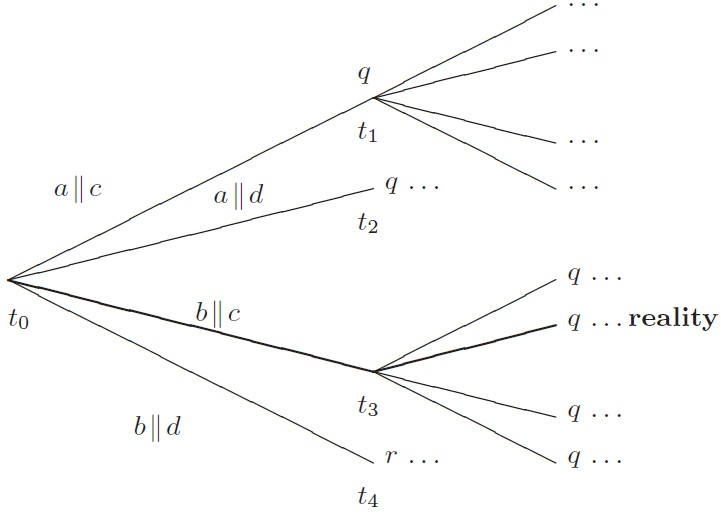
\includegraphics[width=0.6\textwidth]{branching_logic.png}
\label{fig:branching_time}
\end{figure}

Branching temporal and action logic is built on top of both dynamic and linear temporal logics and captures the essential properties of actions and time that are of value in specifying agents. It also adds several specific branching-time operators. $A$ denotes "in all paths at the present moment". The present moment here is the moment at which a given formula is evaluated. $E$ denotes "in some path at the present moment". The reality operator $R$ denotes "in the real path at the present moment". Figure \ref{fig:branching_time} illustrates the example of branching time for two interacting agents.

